\chapter{System}
The software that is used in the autonomous landing system is based on the LSTS toolchain \citep{pinto2013lsts}, with \gls{rtk-gps} solution calculated in RTKLib. The toolchain was developed for support of networked heterogeneous air and ocean vehicle systems. The toolchain supports interactions over wireless network, and is supports interaction with different system responseable for the low end control. The toolchain contain four different modules, namely \gls{imc}, DUNE, NEPTUS and Glued.

DUNE (DUNE Uniform Navigation Environment) is a runtime environment for unmanned systems on-board software written in C++. DUNE is capable to interact with sensors, payload and actuators, in addition to communication, navigation, control, manoeuvring, plan execution and vehicle supervision. The software separate operations into different task that each has there own thread of execution. DUNE apply a message bus that is responsible for forwarding \gls{imc} message from the producer to all registered receivers.

Neptus is a Command and Control software which is used to command and monitor unmanned systems that is written in Java. Neptus is able to provide coherent visual interface to command despite the heterogeneity in the controlled system that it is interacting with.  This allow the operator to command and control unmanned system without the need to dwell into specific command and control software in the unmanned system.
\section{Navigation system}
The navigation system receive state information mainly from the pixhawk, however the the system is able to receive position and velocity from a \gls{rtk-gps} subsystem were the solution is calculated in RTKLib. The system decide if it should use \gls{rtk-gps} through a DUNE task which manage the the source of the navigation data, which will be referred to as the navigation task.

The operator can monitor which source is used in the navigation task through a interface that indicate which source is available.
\subsection{RTK-GPS system}
The navigation system receive its \gls{rtk-gps} solution from a DUNE task, which is connected to the open-source program RTKLib \citep{takasu2009development}. RTKLib contains several separated program that can be used in the field of \gls{rtk-gps}, where the program rtkrcv is used in the \gls{uav} to calculate the \gls{rtk-gps} solution. The program that is used in the base station is str2str, which retrieve the raw data from a GNSS receiver and transmits the data over tcp to the \gls{uav}. The GPS receivers that is used in both the \gls{uav} and base station is a Ublox Lea M8T. The structure of the RTKLib software configured with a rover and base station is shown in figure \ref{figure:RTKLIB_STRUCTURE}.
\clearpage
\begin{figure}[H]
	\centering
		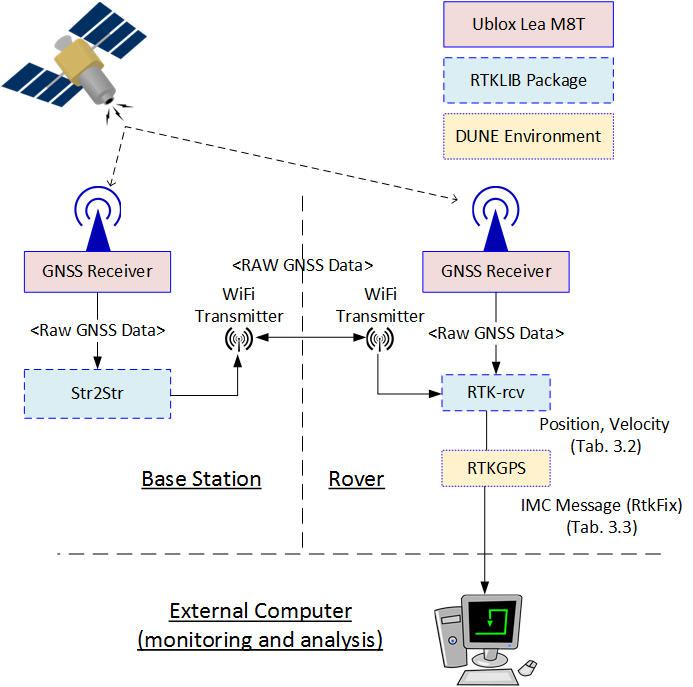
\includegraphics[width=1\textwidth]{figs/RTKLIB.png}
		\caption{The communication structure of \gls{rtklib}}
		\label{figure:RTKLIB_STRUCTURE}
\end{figure}
\clearpage
As part of the \gls{rtk-gps} system the base station has it's own DUNE task running that calculate the position of the base station. The operator has to decide when the the \gls{gps} position of the base station should be considered as fixed, which will result in that the \gls{rtk-gps} DUNE task can include the base station in it's \gls{imc} message. This is require since RTKLib does not include the base position in it's output message. 
\subsection{Navigation source}
The source of the position and velocity solution which is the output from the navigation system is decided in a DUNE task that consume both sensor data from the \gls{rtk-gps} system and the pixhawk. A requirement for use of \gls{rtk-gps} is that the position of the base station is fixed and included in the \gls{imc} message from the \gls{rtk-gps} task, in addition that the operator has decided that \gls{rtk-gps} should be used if available and the \gls{rtk-gps} solution is fixed.

The navigation allows for use of float solution of \gls{rtk-gps} given that it has previous been fixed, for a limited time. 

\subsection{Operator interface}
A interface for navigation source monitoring has been created in Neptus in order to ease monitoring of which source the \gls{uav} is using as position and velocity source. The interfaced apply a color code to indicate which source is currently in use in addition to all sensor system that are available, as seen in table \ref{Tb:Color Code}.

\begin{table}[H]
\begin{center}
    \begin{tabular}{ | l | l |}
    \hline
    \textbf{Color} & \textbf{Description} \\ \hline
    White & Not available \\ \hline
    Yellow & Available, but not in use \\ \hline
    Green & Available, and in use \\ \hline
    \end{tabular}
\end{center}
\caption{Net approach parameters }
\label{Tb:Color Code}
\end{table}

%\subsection{Position correction}%Flytt til resultat
%The highly dynaimcal nature of the uav create a challenge for the navigation system due to the blocking of the gps antenna from the satellite constellation. The problem was reduced by using a gps receiver that has a high performance in satellite tracking, however this does not remove the problem. A float solution from the gps system is valid for some seconds after fix is lost, due to the predictive nature of the Extended Kalman filter in rtklib. However after a seartin amount of time the navigation system swithces over to use the position estimate from the pixhawk, which has a lower accuracy level then the rtk gps system. To increase the accuracy level a offset solution is proposed. By calculating the difference between the fixed rtk gps solution and the position solution from the pixhawk a offset can be found. If the offset can be assumed constant or quasi stationary it can be used to increase to accuracy level for the navigation system enough to allow for completion of critical phases of a manoeuvre. However tests showed that the offset was not constant nor quasi stationary. By applying the offset to the pixhawk position solution the accuracy level will increase, but not enough to allow for execution of critical manoeuvres.
%In order to make the navigation system more robust, some methods was explored. 
\section{Path generation}
The autonomous landing system is designed such that the \gls{uav} is able to landing is a stationary or moving net. This thesis will focus on landing in a stationary net, however the system that has been created can be used to land into a moving net. To be able to hit the net a virtual run way is created as a glide slope towards the net, which is divided into four phases. This phase will be described in section \ref{SS:netApproach}.

In order of start the landing approach the \gls{uav} must be at the correct height in order to start the approach toward the net. Therefore a plan has to be created such that the \gls{uav} is able to reach the correct height in a controlled manor. The plan that creates a path for the \gls{uav} is described in section \ref{SS:LandingApproach}.

The operator should be able to control all parameters which is critical for the path generation. This is done through Neptus, where a plugin is used for parameter setting and plan generation. The plug-in is described in section \ref{SS:PlanGeneration}.


The landing plan is design with the assumption that the aerial space in which the uav operates is limited. The limitation can be the range of the uav, regulatory limits or weather. In addition the autonomous landing system must be able to perform a safe landing from any initial position. Furthermore the size of the virtual run way should be constructed by the operator. The type of uav operation dictates the maximum size of the landing path. Different types of uav operation is LOS, ELOS, BLOS and BRLOS. Only the first is considered in this thesis, which means that the pilot must have the uav in view during the entire flight. The operator must also be able to control the angle which the uav is descending, which means that the height of the landing path is fixed. Therefore the uav must be at the correct altitude before it can start descending toward the landing net.

A landing plan that is proposed consist of Dubins path \ref{S:DubinsPath} in the lateral plane, and straight lines in the longitudinal plane. The path is generated from an arbitrary start positing, and will create a continuous path toward the landing approach. The design is inspired by the work done in \citep{Skulstad&Syversen} were way-points was used to guide the uav toward the landing approach.

The plan is generated in a Dune task which receive a plan generation request from Neptus. Then a plan is created, which is sent to the Dune task Plan manager, which in turn sent desired state to the guidance system. The plan is decoupled from the guidance system, which allow for use of different control design when executing the landing plan.

The Dubin path is constructed with a followPath manoeuvre.

The landing plan generated by the Dune task can be requested for review by the operator in Neptus. The plan will not start before the operator has reviewed the plan, and approved by uploading it to the uav. In the uploaded version a specification list on which controller that should be used is included.  
\subsection{The net approach}\label{SS:netApproach}
The net approach path is inspired by the work done in \citep{Skulstad&Syversen} where waypoint was used to create a straight line path towards the net. This method proved successful, and since the \gls{uav} descent towards the net should be as controlled as possible only small angles is used when transitioning between waypoints. Figure \ref{Fig:LandingPhase} shows the approach towards a stationary net. The landing phase consist of four way points which is defined relative to the position of the net. The four way-points in the net approach is defined as follows:
\begin{subequations}
\begin{align}
&\mathbf{WP1} = 
\begin{bmatrix}
-a0 \\
0 \\
h_{nc} + a1\tan(\gamma_a) 
\end{bmatrix}\\
&\mathbf{WP2} = 
\begin{bmatrix}
a1 \\
0 \\
h_{nc} - a1\tan(\gamma_a)
\end{bmatrix}\\
&\mathbf{WP3} = \mathbf{WP2} + 
\begin{bmatrix}
a2 \\
0 \\
a2\tan(\gamma_d)
\end{bmatrix}\\
&\mathbf{WP4} = \mathbf{WP3} + 
\begin{bmatrix}
a3 \\
0 \\
0 \\
\end{bmatrix}
\end{align}
\end{subequations}
were the description of the parameters used is given in table \ref{Tb:Approach Parameters}. The net is placed between the first and second way points such that transitional behaviour do not occur during the finale stage of the net landing. In addition the path has been made with the assumption that the $\gamma_a$ and $\gamma_d$ is considered small. This assumption is made to easy the demand of the controllers used in the landing system.
\begin{table}[H]
\begin{center}
    \begin{tabular}{ | l | l |}
    \hline
    \textbf{Parameter} & \textbf{Description} \\ \hline
    $a0$ & The distance behind the net \\ \hline
    $a1$ & The distance in front of the net \\ \hline
    $a2$ & The length of the glide slope \\ \hline
    $a3$ & The length of the approach towards the glide slope \\ \hline
    $\gamma_a$ & The net attack angle \\ \hline
    $\gamma_d$ & The glide slope angle \\ \hline
    \end{tabular}
\end{center}
\caption{Net approach parameters }
\label{Tb:Approach Parameters}
\end{table}
The way point vectors are rotated into the NED frame by a rotation around the z-axes.
\begin{equation}
WP^n = R(\psi_{net})WP^b
\end{equation}
were $\psi_{net}$ is the heading of the net, and $R(\psi_{net})$ is the rotation matrix around the z-axis.
\begin{figure}\label{Fig:LandingPhase}
\def\svgwidth{\textwidth} % Defining the width since Inkscape hasn't done this yet in the .pdf_tex file
\input{InkFig/LandingPhase.pdf_tex}
\end{figure}

\subsection{The landing path approach}\label{SS:LandingApproach}
Before the \gls{uav} can start its decent towards the net it must be at the correct height with correct orientation, which is defined by the length of the run way, in addition to the chosen decent angle. The \gls{uav} should also achive this goal in a controlled manor where the decent it limited to a given decent angle. This is a requirement from any initial position. In addition it's an advantage for the control system if the lateral path is smooth enough for path following purpose.

The lateral path was chosen for the autonomous landing system is Dubins path, due to it's simplicity in description and it fulfils the requirement that it's smooth enough for path following. Since it's desired for the \gls{uav} to decent with small decent angle the longitudinal path is constructed with straight lines. Combined with Dubins path, the circles in the start and end of the path becomes spirals. This increase the demands on the controllers used, since they has to both control the heading in addition to the decent rate with the same control surface. This is the main reason for small angles in the longitudinal path.

The path generation system is designed such that the operator can choose how the path should be generated. The system allows for manual creating of the path, or simply create the shortest path from the start pose to the end pose, which is the first way-point in the path towards the net.
\subsubsection{Shortest path}
When the operator decide that the path should be generated automatically the shortest path from the initial pose to the first way-point is calculated. This is done by calculating all four variants of Dubins path, which is given in table \ref{Tb:DubinsTurningDirection}. After the length of each path is calculated, where the shortest path is chosen to be the landing path.
\subsubsection{Manual path}
If the path should be generated manually the operator has to decide the start and end turning directions.
One mode allow for manual deciding which side the start and finish circle should be in respect on the start pose, and the net landing approach. This allow the operator full control over the landing path, and can choose a landing path that is operation feasible and not necessary the shortest path.
\subsubsection{Longitudinal path}
A desired behaviour in the lateral plane is that the \gls{uav} should have a controlled decent. Given this desired behaviour it was decided that the lateral plane should be a glide slope, which means that the decent angle can be considered small. The strategy chosen to solve this problem is the use of straight lines in the lateral plane. The straight lines are is included with Dubins path such that the turn in Dubins path becomes a spiral.

At the end of Dubins path the path is checked if the correct height has been reach. If the correct height has not been reached the path will create a spiral that converge to the correct height. When the correct height has been reach a last arc is created in order for the \gls{uav} to get the correct orientation.
\subsection{Transition into the net approach}
In order to fully control when the \gls{uav} should start its decent the landing plan can include a loiter at the end of the approach. The loiter manoeuvre can be enabled such that the operator is able to make final preparation with the runway, or used together with a moving net to ease coordination. The loiter manoeuvre is exited when a end manoeuvre signal is sent from Neptus.
\subsection{Plan generation}\label{SS:PlanGeneration}
The plan is configured and generated thought a plug-in in Neptus. In the plug-in the operator can choose how the plan should be generated, as well as the length of the run way and the desired decent rate.
\section{Guidance and control system system}
The guidance system consist of two part. Sliding mode controller, and a los controller

\subsection{Sliding mode controller}
For course control the system use a sliding mode controller that was proposed in the paper \citep{fortuna2015cascaded}, which USGES stability property.